\begin{frame}{Updates}
  \begin{itemize}
    \item Did not make submission deadline for MobiSys
    \item Submit to imwut instead (12/15)
    \item Approx. 7500 Lasers labeled
    \item Approx. 150 Fish labeled
  \end{itemize}
\end{frame}

\begin{frame}{Laser Results}
  \centering
  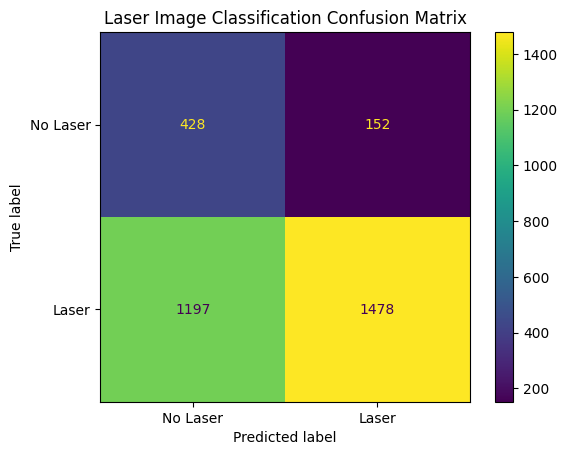
\includegraphics[height=0.7\textheight,width=0.49\textwidth,keepaspectratio]{images/a3d-laser-confusion.png}
  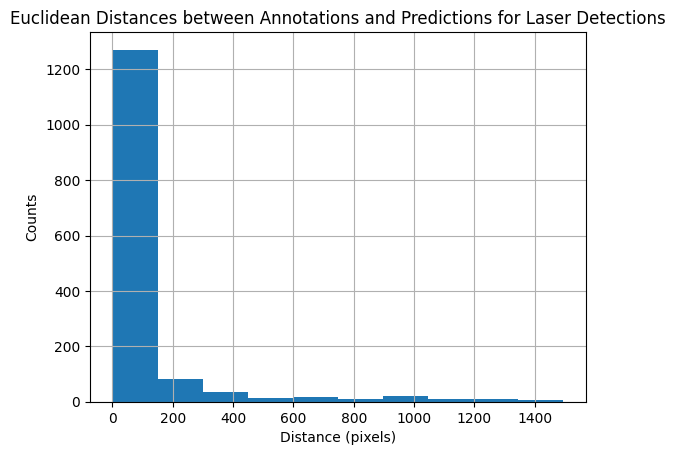
\includegraphics[height=0.7\textheight,width=0.49\textwidth,keepaspectratio]{images/a3d-laser-error.png}
\end{frame}

\begin{frame}{Raw Improvements}
  \centering
  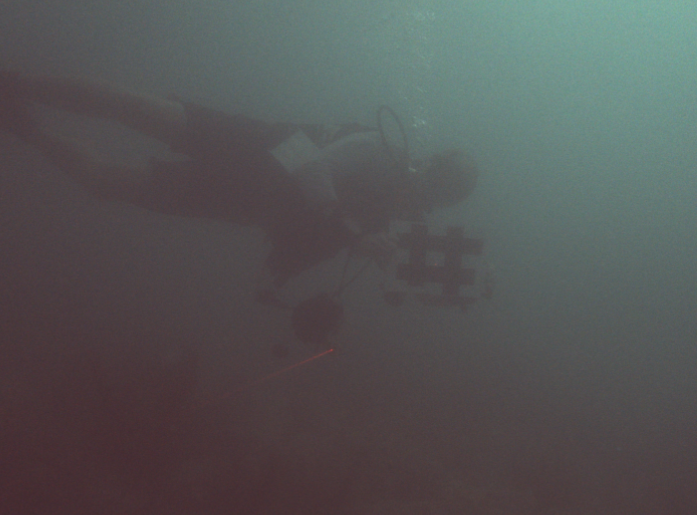
\includegraphics[height=0.7\textheight,width=0.49\textwidth,keepaspectratio]{images/a3d-diver-old-raw.png}
  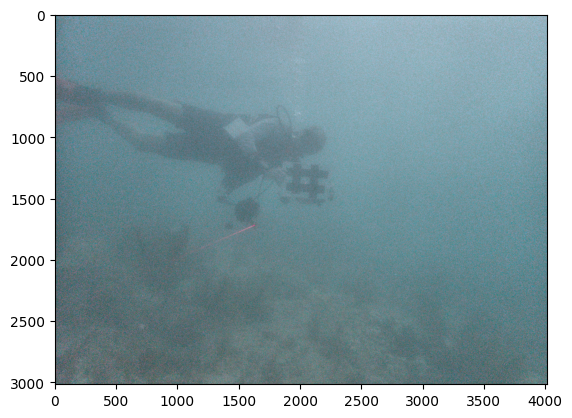
\includegraphics[height=0.7\textheight,width=0.49\textwidth,keepaspectratio]{images/a3d-diver-no-seathru.png}
\end{frame}

\begin{frame}{Sea Thru}
  \centering
  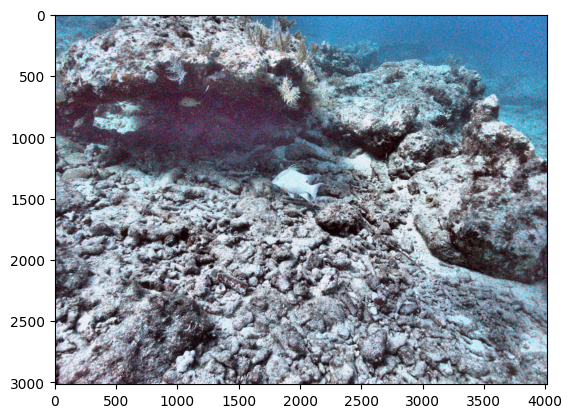
\includegraphics[height=0.7\textheight,width=0.49\textwidth,keepaspectratio]{images/a3d-seathru.png}
  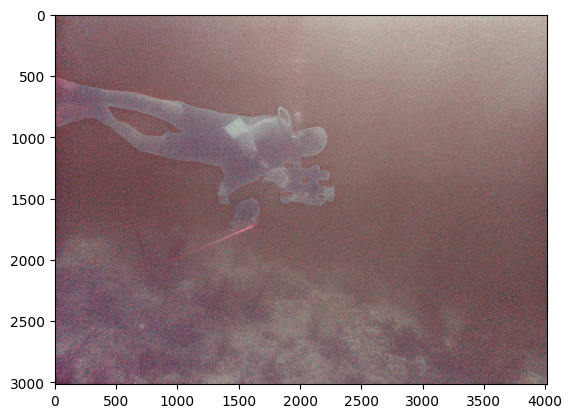
\includegraphics[height=0.7\textheight,width=0.49\textwidth,keepaspectratio]{images/a3d-diver-seathru.png}
\end{frame}

\begin{frame}{Sea Thru}
  \centering
  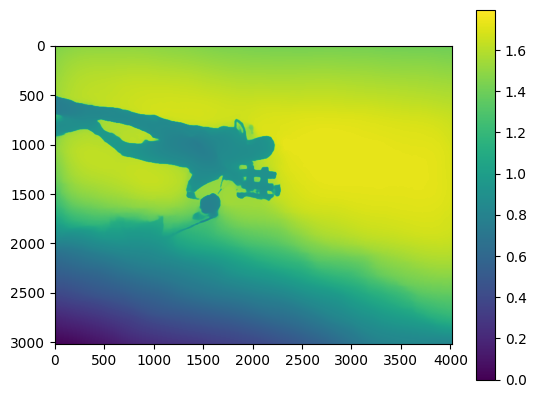
\includegraphics[height=0.7\textheight,width=0.49\textwidth,keepaspectratio]{images/a3d-diver-depth.png}
  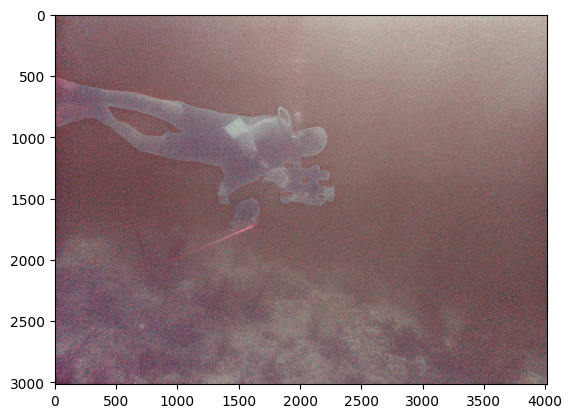
\includegraphics[height=0.7\textheight,width=0.49\textwidth,keepaspectratio]{images/a3d-diver-seathru.png}
\end{frame}

% Slides for 2024-11-14
% To create a slide, use the following:
% \begin{frame}{TITLE}
%     BODY
% \end{frame}

% To create a slide with a bullet list, use the following:
% \begin{frame}{TITLE}
%     \begin{itemize}
%         \item ITEM 1
%         \item ITEM 2
%     \end{itemize}    
% \end{frame}

% To create a slide with numbered list, use the following:
% \begin{frame}{TITLE}
%     \begin{enumerate}
%         \item ITEM 1
%         \item ITEM 2
%     \end{enumerate}
% \end{frame}

% To create a slide with a graphic:
% 1. Add the graphic to this folder (named picture.png)
% 2. Use the following:
% \begin{frame}{TITLE}
%     \centering
%     \includegraphics[height=0.7\textheight,width=0.7\textwidth,keepaspectratio]{picture.png}
% \end{frame}

% To create a slide with two columns, use the following:
% \begin{frame}{TITLE}
%     \begin{columns}
%         \begin{column}{0.5\textwidth}
%             COLUMN 1 BODY
%         \end{column}
%         \begin{column}{0.5\textwidth}
%             COLUMN 2 BODY
%         \end{column}
%     \end{columns}
% \end{frame}
